\documentclass[10pt,twocolumn]{article}
\usepackage{geometry} 
\geometry{letterpaper} 
\usepackage[parfill]{parskip}    % Activate to begin paragraphs with an empty line
\usepackage{wrapfig}
\usepackage{graphicx,subfigure}
\usepackage{amssymb}
\usepackage{epstopdf}
\usepackage{subfigure}
\usepackage{color}
\usepackage{cite}

\DeclareGraphicsRule{.tif}{png}{.png}{`convert #1 `dirname #1`/`basename #1 .tif`.png}
 
\oddsidemargin=-0.01in
\evensidemargin=-0.01in
\topmargin=-0.5in
\textheight 8.9in
\textwidth 6.5in

\newcommand {\vct}[1]{\mbox {\boldmath $#1$}}
\newcommand {\tDelta} {\mbox {\tiny $\Delta$} }

\usepackage{titlesec}

\begin{document}
\bibliographystyle{unsrt}
\pagenumbering{arabic}
\pagestyle{plain}

\def\bfi{\begin{figure}[h]} \def\efi{\end{figure}}
\def\bfit{\begin{figure}[t]}   \def\efi{\end{figure}}
\def\bfib{\begin{figure}[b]} 
\def\bfih{\begin{figure}[htb]}
\def\bfip{\begin{figure}[p]}
\def\be{\begin{equation}} \def\ee{\end{equation}}
\def\bfi{\begin{figure}[p]} \def\efi{\end{figure}} 
\def\bi{\begin{itemize}} \def\ei{\end{itemize}}
 
\definecolor{bl}{rgb}{0.,0.2,0.6}
\definecolor{red}{rgb}{1.0,0.0,0.0}

\titleformat{\section}
{\color{bl}\normalfont\Large\bfseries}
{\color{bl}\thesection}{1em}{}

\titleformat{\subsection}
{\color{bl}\normalfont\large\bfseries}
{\color{bl}\thesubsection}{1em}{}

\titleformat{\subsubsection}
{\color{bl}\normalfont\large\bfseries}
{\color{bl}\thesubsubsection}{1em}{}

\def\be{\begin{equation}} \def\ee{\end{equation}}
\def\bfi{\begin{figure}[p]} \def\efi{\end{figure}} 
\def\bi{\begin{itemize}} \def\ei{\end{itemize}}
\def\bea{\begin {eqnarray}}  \def\eea{\end {eqnarray}}

\newcommand{\ovl}{\overline}
\newcommand{\lal}{\langle}
\newcommand{\ral}{\rangle}

\title{\Large \bf \color{bl} The Johns Hopkins Turbulence Databases, an Open Simulation Laboratory for Turbulence Research} 
\author{\bf Kalin Kanov, Randal Burns, Cristian Lalescu \& Gregory Eyink} 
\baselineskip=.18in
  
\twocolumn[\maketitle]

\setcounter{page}{1}

The Johns Hopkins Turbulence Databases are an open simulation laboratory for the study of turbulence. They provide an immersive environment, in which
world-class numerical simulation datasets are available ``at your fingertips". Such an environment has the potential to transform our understanding of
turbulent flows.

 
\vspace{-0.2in}
\section{Introduction}
\label{sec-introduction}
\vspace{-0.15in}

Most, if not all, science disciplines have developed computational branches. Examples include computational physics, computational biology,
computational chemistry, computational fluid dynamics, and others. In some cases experimentation is simply not possible as is the case in cosmology.
In others experimentation may be too expensive or too dangerous. In the case of fluid dynamics and turbulence research in particular direct numerical
simulations (DNS) are widely adopted tools for the development and refinement of turbulence models, which improve our understanding of how the
underlying physical processes work. The Navier-Stokes equations, which govern
turbulent fluid flow, are discretized and integrated forward in time, solving for physical field variables (e.g. velocity and pressure) as function of space 
and time in the domain of the simulation. 

The memory and computational requirements of DNS of turbulence scale as the third and fourth power of the
non-dimensional Reynolds number, \emph{Re} \cite{Lee}. Turbulent flows of practical interest usually have high
\emph{Re}, and must therefore be solved using supercomputers. Preparing and running such a simulation requires substantial expertise in parallel
computing and turbulence research, but moreover it requires access to a supercomputing facility. Traditionally, such undertakings have been team 
efforts that are planned and prepared for ahead of time, the particular science questions to be answered have been thought of in advance and most of the
analysis is done during the simulation. Only representative snapshots are stored for subsequent analysis and even if more data are available accessing
them is often not easy and usually entails the downloading of large amounts of data to a local machine. In order to provide access to high-quality
world-class turbulence DNS data to researchers that may not have access to supercomputing facilities and the public as a whole, our group at Johns 
Hopkins has developed an open turbulence laboratory, the Johns Hopkins Turbulence Databases (JHTDB). 

Here, we describe our experience building and operating the JHTDB and our efforts to provide ``at your fingertips" access to terabyte simulation datasets
to anyone in the world with an internet connection. An open simulation laboratory complements the DNS approach to the study of turbulence. The entire
space-time history of landmark simulations are stored persistently in a database cluster. Coupled with built-in analysis functionality this allows researchers
with modest computational and storage capabilities to perform sophisticated analysis using high-resolution datasets, traverse the flow both forward and
backward in time, repeat and refine experiments, tune the parameters of their analysis routines, test new hypothesis and use the data in ways, which were 
not even envisioned when the simulations were run. Additionally, an open simulation laboratory can be used for teaching and training the next generation 
of researchers.

The deployment of an open simulation laboratory for turbulence research has already transformed our understanding of turbulence and has allowed for new
types of analysis to be performed in this environment. Particles immersed in the simulated flow can be tracked both forward an backward in time. 
Ensembles of particles are evaluated together and the experiments can be repeated multiple times to achieve the required confidence in the results.
Analysis of this type was carried out in magnetohydrodynamics (MHD), where stochastic trajectories arriving at a point $(x, t)$ were traced backward in 
time to the initial time, $t_0$ and the magnetic field was then transported forward along the trajectories to the point $(x, t)$. This numerical experiment has
revealed why magnetic field-lines in solar flares break and reconnect in as little as 15 minutes as opposed to the millions of years predicted by classical 
theory \cite{Eyink}.

The great advances in computing capabilities of the recent past have led to scientific datasets of unprecedented size. The standard DNS of turbulent flows
produce datasets that are 10s to 100s of terabytes, while leading-edge simulations have already crossed the petabyte threshold \cite{Lee}. The rate at
which new datasets are generated is also accelerating. This highlights the enormity of the task at hand, to persistently store large datasets, provide public access
to them and ensure that they can be analyzed in an efficient manner. 

\section{JHTDB Overview}

The JHTDB was designed to provide efficient yet flexible access to world-class high-resolution turbulence DNS data \cite{Yi, Perlman}. Over the past
several years since its inception in 2007 some aspects of the architecture were modified, new analysis functionality was added and new ways of accessing
the data were provided. We provide an overview of the architecture and summarize some of these developments here.

The JHTDB currently stores four datasets, which are the output of DNS of four types of turbulent flows. This includes: 
\begin{itemize}
\item a forced isotropic turbulence dataset on $1024^4$ space-time data points at a Taylor-scale Reynolds number of $Re_{\lambda} = 433$;
\item a steady-state incompressible magnetohydrodynamic (MHD) turbulence dataset on $1024^4$  space-time data points, forced with a Taylor-Green flow,
with $Re_{\lambda , u} = 186$  and $Re_{\lambda , b} = 144$ for the velocity and magnetic field, respectively;
\item a channel flow dataset at $Re_\tau = 1000$ on $2048 \times 1536 \times 512$ spatial data points and 4000 time steps;
\item a variable-density mixing flow dataset on $1024^3$ spatial data points and 1015 time steps.
\end{itemize}
The total amount of space occupied by these datasets is over 200TB. The data are partitioned spatially and temporally across a cluster of relational
databases. The database nodes are part of the 1.1PB GrayWulf cluster \cite{Szalay} and the 11PB DataScope cluster (http://idies.jhu.edu/datascope) at JHU.
Each node runs Microsoft SQL Server and provides built-in analysis functionality, implemented as user-defined functions or stored procedures in the
Common Language Runtime (CLR). The data and analysis functionality are accessible through a Web-server front end (http://turbulence.pha.jhu.edu), 
which provides Web-services implemented using the SOAP protocol (Simple Object Access Protocol), a cutout service producing HDF5 files of the raw
simulation data and a Web-query interface. Users can access the Web-services directly or through several client libraries, which we have provided, 
including Matlab, C, Fortran and Python wrappers. The architecture of the JHTDB is shown in Figure \ref{fig:architecture}.

\begin{figure}
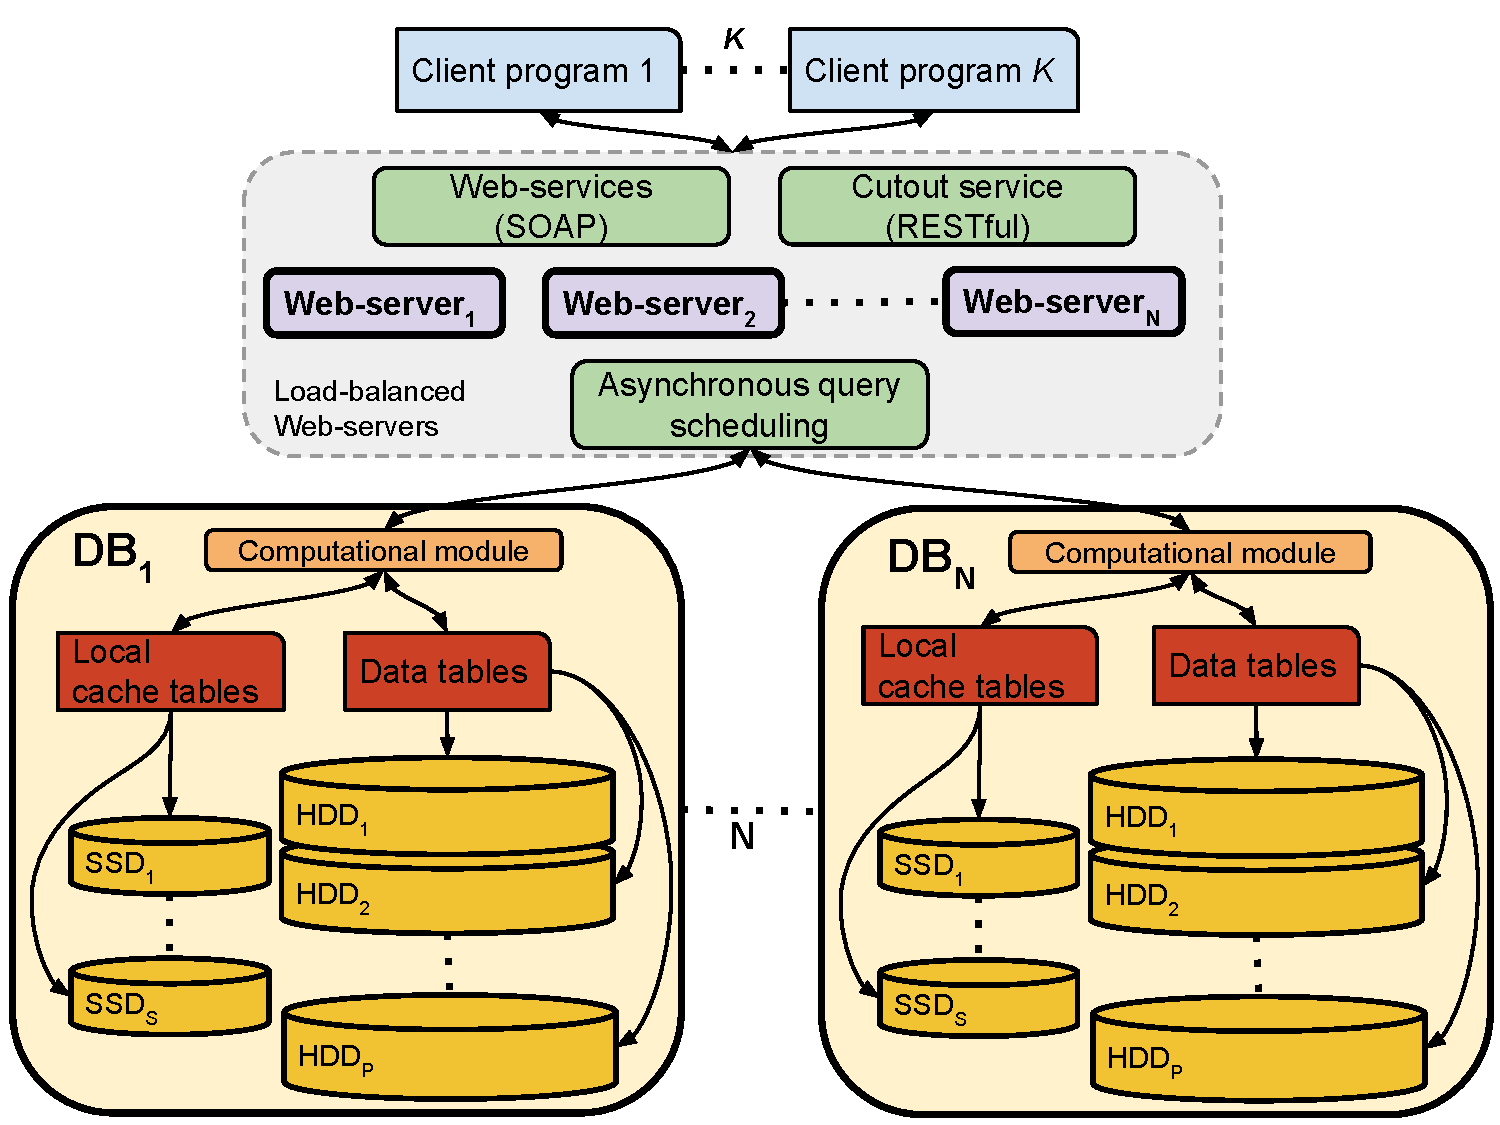
\includegraphics[width=0.6\textwidth]{jhtdb_diagram.pdf}
\caption{Architecture of the JHTDB.}
\label{fig:architecture}
\end{figure}

The analysis functions used in turbulence research are data-intensive, they operate over collections of points and to compute the result at each target point
they access a large number of neighboring data points. Some functions are also data-reducing, they evaluate or compute over a large number of data
points, but produce smaller result sets. These types of computations are much more efficiently executed on the servers near the data. Large amounts of data
do not have to be moved across the network and the computations can be evaluated in a distributed manner across the nodes of the cluster. However, the
functionality provided to the users should also be general enough to allow for different types of analysis and customization of experimental parameters.
With these considerations in mind, we have developed Web-services methods that evaluate simulation parameters on a set of target locations. Users of 
the JHTDB can request the following:
\begin{itemize}
\item values of the simulation fields on and off the grid (locations off the grid are interpolated using Lagrange and spline polynomials of varying orders);
\item first and second order derivatives of the simulation fields evaluated using finite-differencing schemes of varying orders;
\item filtered quantities, such as the filtered velocity, filtered velocity gradient, sub-grid stress tensor, etc. (filtering is performed using a box filter);
\item the positions of particles tracking the simulated flow (particle tracking is performed using a second order accurate Runge-Kutta integration scheme);
\item all values of the simulation fields and derived quantities above a prescribed threshold (derived quantities currently include the vorticity and Q-criterion).
\end{itemize}

In order to amortize I/O, improve the specificity of reads and reduce the overhead of indexing the data, we partition the data into data cubes or ``atoms".
The atoms are represented as binary-large objects (or BLOBs) in the database tables. Each is of size $8^3$ data points and stores the data for one of the
simulation fields (e.g. velocity or pressure). Most of the computations require data from the immediate neighborhood of the target location (e.g. a cube
centered on the target location) as a kernel. The size of each kernel depends on the parameters of the request, but is usually in the $4^3$ to $8^3$ range.
Additionally, given a size of $8^3$ data points for a data atom, each record fits within a single database page. This allows us to obtain the data for each
computation with a small number of I/Os.

\begin{figure*}
\frame{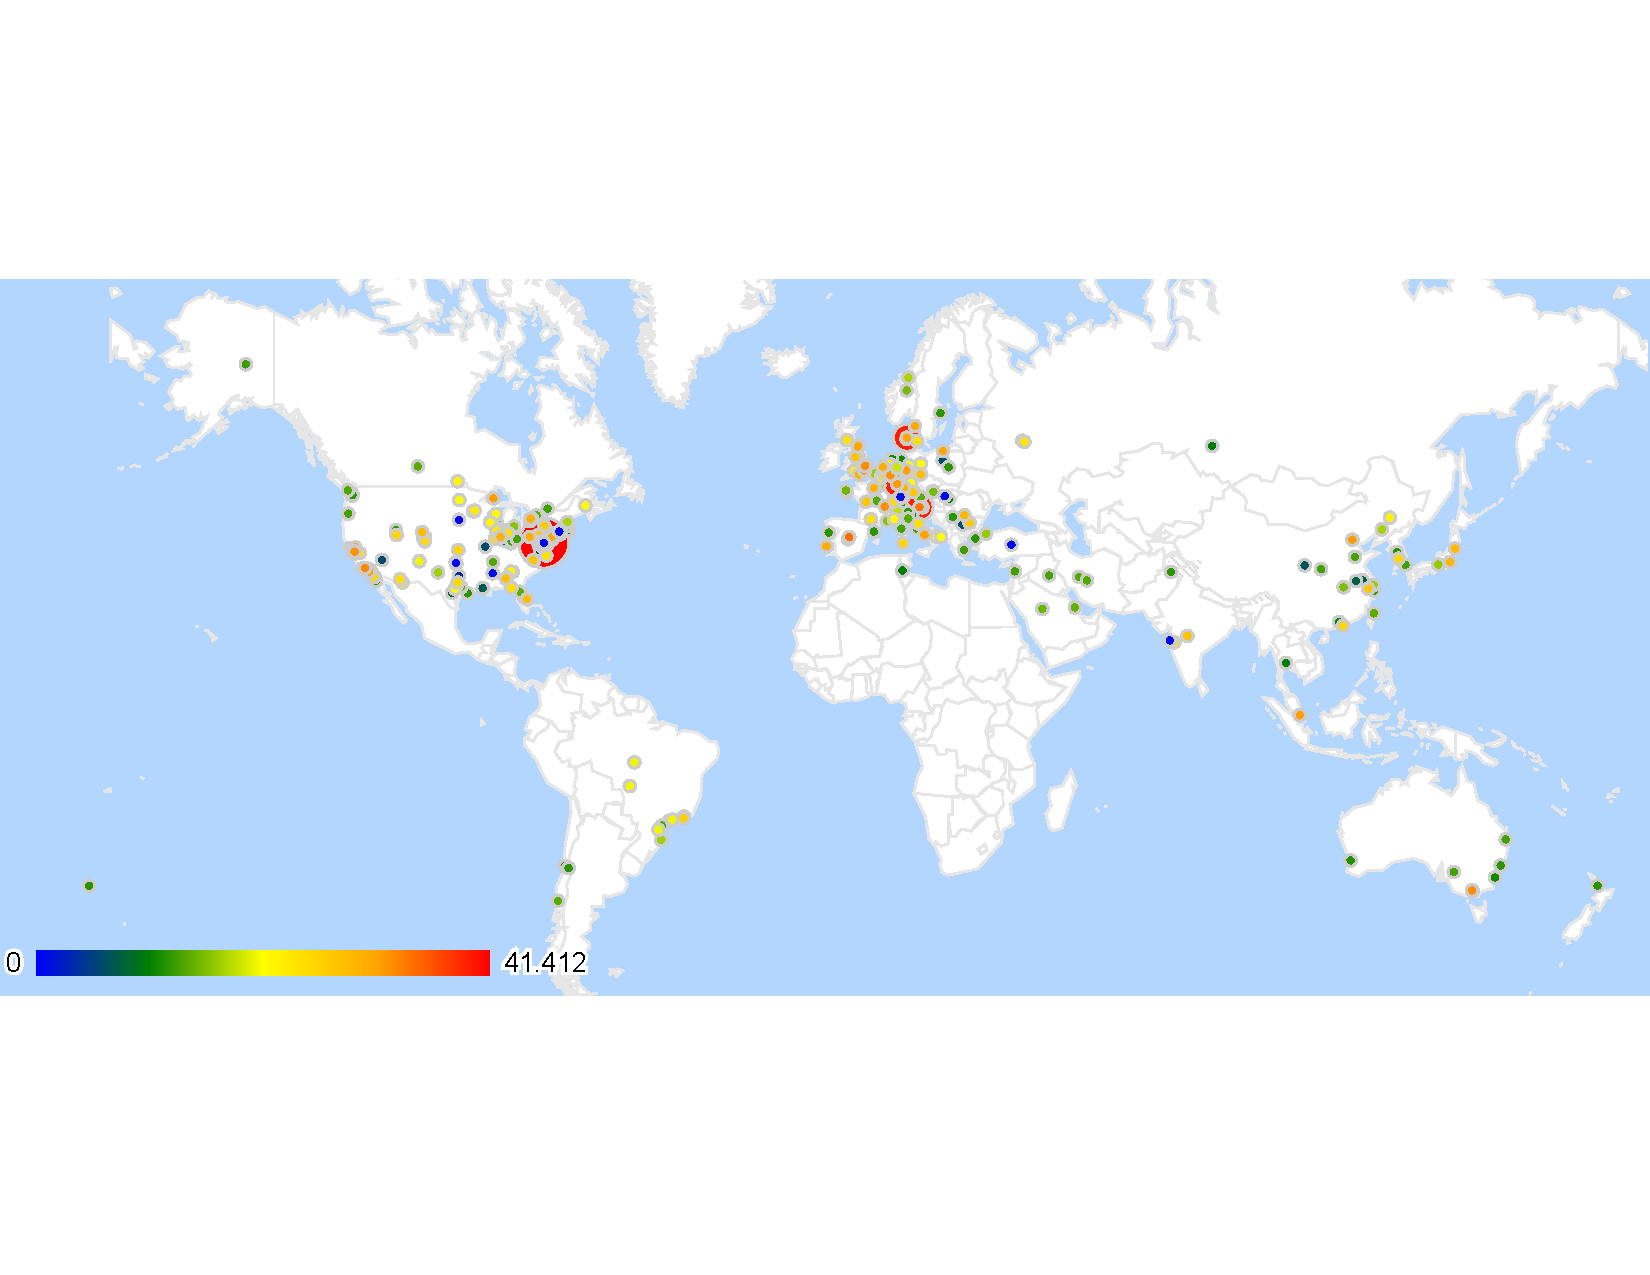
\includegraphics[width=1.0\textwidth]{ip_map.pdf}}
\caption{Origin location of queries to the JHTDB. Each IP address location is colored based on the total number of points queried in log scale.}
\label{fig:ip_map}
\end{figure*}

The database atoms are indexed and distributed across the nodes of the database cluster by means of the Morton z-order space-filling curve (Z-curve). The 
Z-curve maps the 3D data to the one dimensional index space. It passes through each location in space once and only once, it is easy to compute and
provides good spatial locality. Spatial locality is important as data points in close proximity in physical space are usually accessed at the same time for the
typical usage patterns of the database.

The Web-services methods provide the commonly used, essential building-blocks of many different scientific experiments. At the same time they
encapsulate the data-intensive portions of these computations. We have developed an I/O streaming framework for the evaluation of kernel computations of
linear-sums \cite{KanovSC11}. In this framework a batch query consisting of multiple target locations is evaluated during a single sequential stream over 
the data. Each computation of a linear-sum can be broken down into partial-sums, which allows us to use an I/O stream, without having to do random 
accesses or keep a large amount of data in memory. The I/O streaming framework is used for the evaluation of interpolation, differentiation and filtering.

In the case of spatial filtering, for certain workloads further optimizations of the evaluation strategy are possible. Workloads that distribute target locations
densely in space and specify large filter widths share not only data, but also computation. A box filter is evaluated by computing the average of all data
points within the filter kernel, which of course makes use of the sum of all data points within the kernel. Therefore, precomputing these sums allows us to
evaluate the box filter at each target location by looking up only eight points in the precomputed ``summed-volumes" dataset \cite{KanovSC12}.

Another interesting type of query, which the JHTDB provides is the threshold query. Such queries are highly data-reducing, they usually have to examine an
entire simulation time-step and produce only the points, whose values are above a prescribed threshold. Their evaluation is complicated further by the fact
that scientists are usually interested in not just the simulation fields, but also derived fields, such as the vorticity, electric current, second and third invariants
of the velocity gradient and others. In order to preserve the computational effort of the evaluation of threshold queries of derived fields we store their results
in a cache database, which resides on solid-state drives (SSDs) attached to each database node. Subsequent queries can be answered from the cache
if they specify the same or higher threshold, are within the same spatial region and are querying the same dataset, field and time-step.

The JHTDB also provides a cutout service, which allows users to obtain the raw simulation data in familiar HDF5 format. The cutout service includes an
option to obtain the raw data by specifying a stride or a step and optionally a filter width. 
In that case a coarser version of the data are produced and if the filter width is larger than a single data point the data are filtered using a box filter. 
For reasonable values of the stride parameter producing a filtered version of the data is only slightly slower than obtaining the raw data through strided access.  
This is because the access is limited by I/O and the transfer of results to the user is limited by network speed. 
The filtering computation introduces a small overhead mainly due to the fact that the data have to be converted
from binary to single precious floating point format to perform the filtering computations.

The evaluation of all queries submitted to the JHTDB is distributed across the nodes of the database cluster and we create multiple connections to each
node in order to exploit the nodes' multicore architecture. The Web-server handling a user request acts as a mediator. It distributes the input across the
database nodes based on the spatial and temporal partitioning of the data and initiates the processing on each node asynchronously. The partial-sum
computations naturally support distributed evaluation and eliminate the need
for replicating data across database node boundaries. The Web-server mediator simply adds the partial results from two or more nodes to produce the
final result. Similarly, the list of points above the user specified threshold produced by each database node are merged by the Web-server mediator. 
Thus, the threshold query result cache is also distributed across the database nodes, which allows it to scale-out as the cluster grows.

\section{Impact of the JHTDB}

\begin{figure*}
\centering
\subfigure[Number of queries]{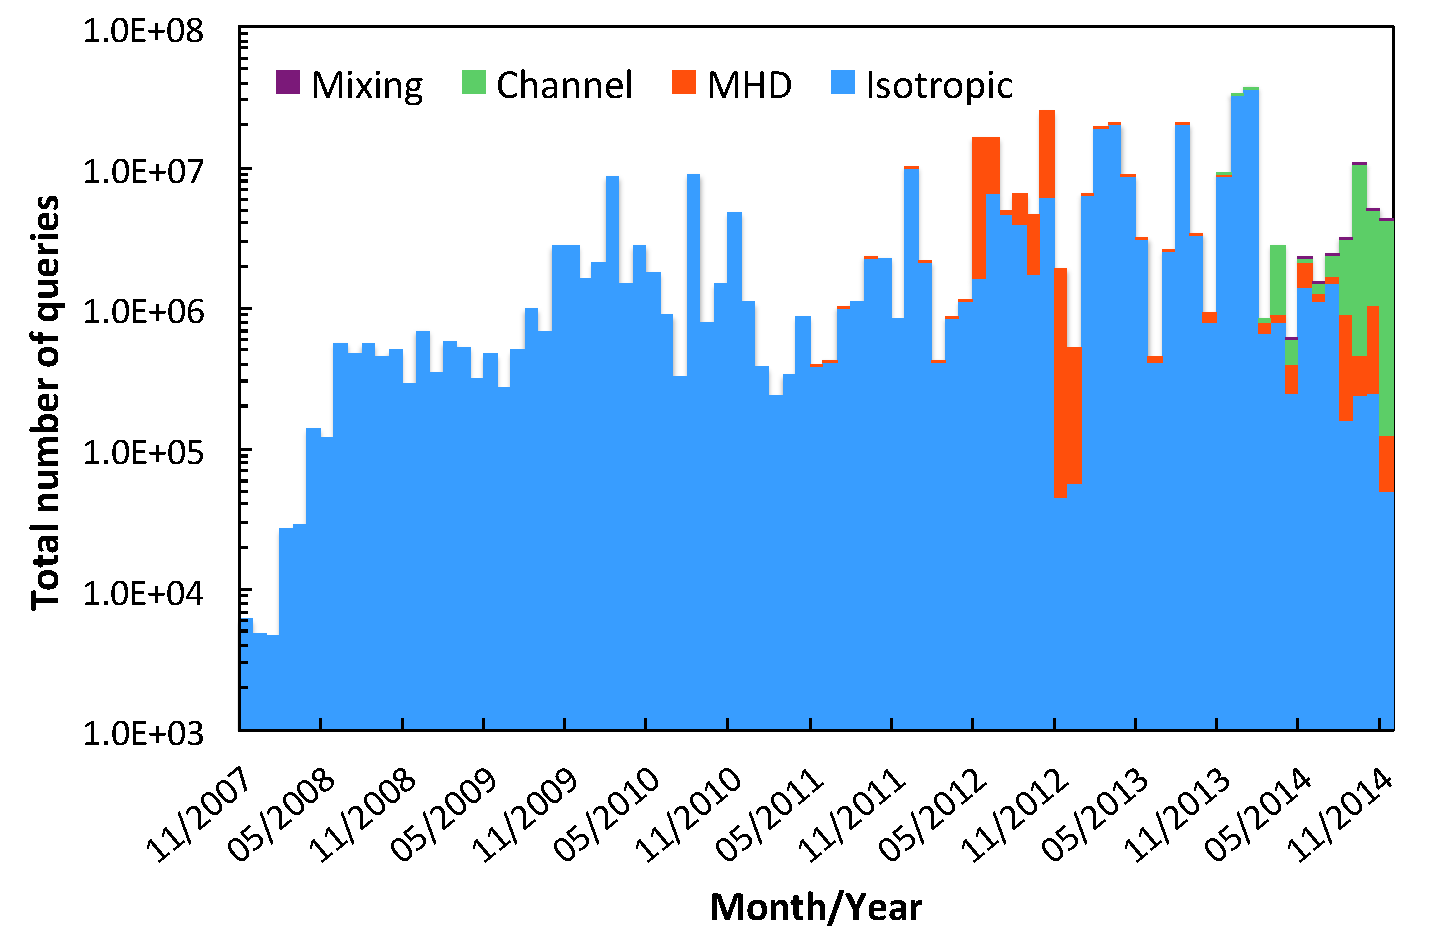
\includegraphics[width=0.49\textwidth]{jhtdb_queries.pdf}\label{fig:queries}}
\subfigure[Number of data points queried]{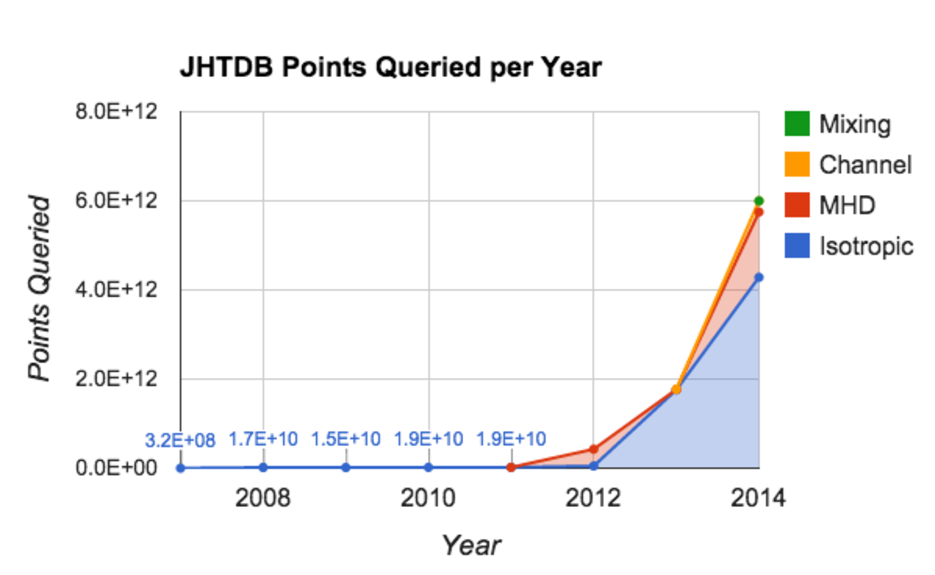
\includegraphics[width=0.49\textwidth]{jhtdb_usage.pdf}\label{fig:points_queried}}
\caption{Semi-log plot of the number of queries and number of data points queried from the JHTDB per year.}
\label{fig:usage}
\end{figure*}

As of the writing of this article the JHTDB has served queries to nearly 12 trillion data points. This serves as a testament to the demand for such high-quality
data and their potential for reusability. Each of the four datasets stored in the JHTDB currently has on the order of a trillion space-time data points. Storing
these data in an open simulation laboratory preserves the computational effort used to generate them, allows for repeatability of experiments and 
verification of results and enables users to come back to the same place in space and time. The continued exploration of the same place in space and 
time produces the same exact data, but users can look at it from different angles, requesting derivatives, spatially filter the data or compute more 
complicated quantities. 
This builds physical intuition about the nonlinear dynamics of the complex flow phenomena and can lead to new discoveries. 

The availability of an open simulation laboratory for the study of turbulent flows has already had a major impact on turbulence research and education. 
The JHTDB has over 150 registered users and queries have been made from over 1500 distinct ip addresses across the globe (Fig. \ref{fig:ip_map}).
Data from the service have been used fully or partially in multiple research projects resulting in at least 40 peer-reviewed publications, including in
high-profile venues such as Nature \cite{Eyink}, Proceedings of the National Academy of Sciences \cite{xu2014flight}, 
and Physical Review Letters \cite{gustavsson2014tumbling, jucha2014time}. 
The impact of the JHDTB has extended to the classroom as well. The laboratory has been used in various classes and student workshops 
around the world (e.g. the ``Tutorial School on Fluid Dynamics: Topics in Turbulence" held at the University of Maryland College Park - 
see http://www2.cscamm.umd.edu/programs/trb10/, to be repeated in the summer of 2015).

\begin{figure*}
\centering
\subfigure[Percentage of queries per query type]{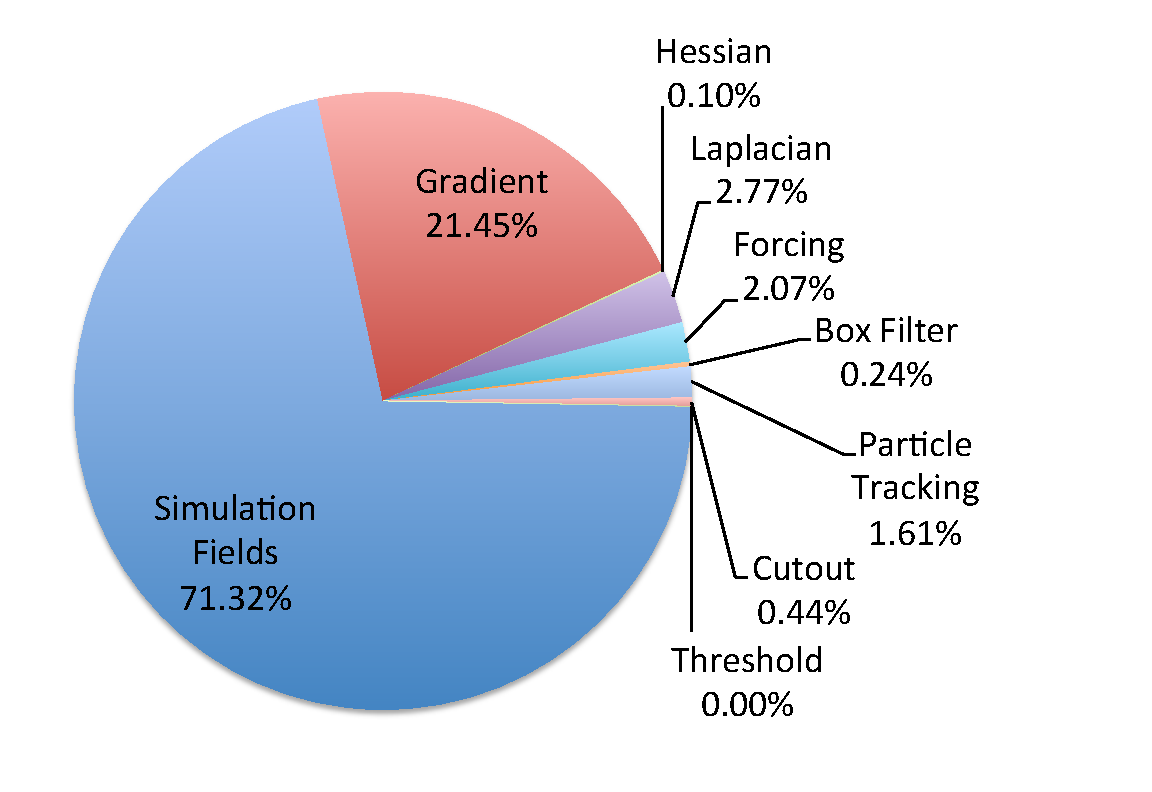
\includegraphics[width=0.49\textwidth]{jhtdb_query_types.pdf}\label{fig:queries_per_type}}
\subfigure[Percentage of data points queried per query type]{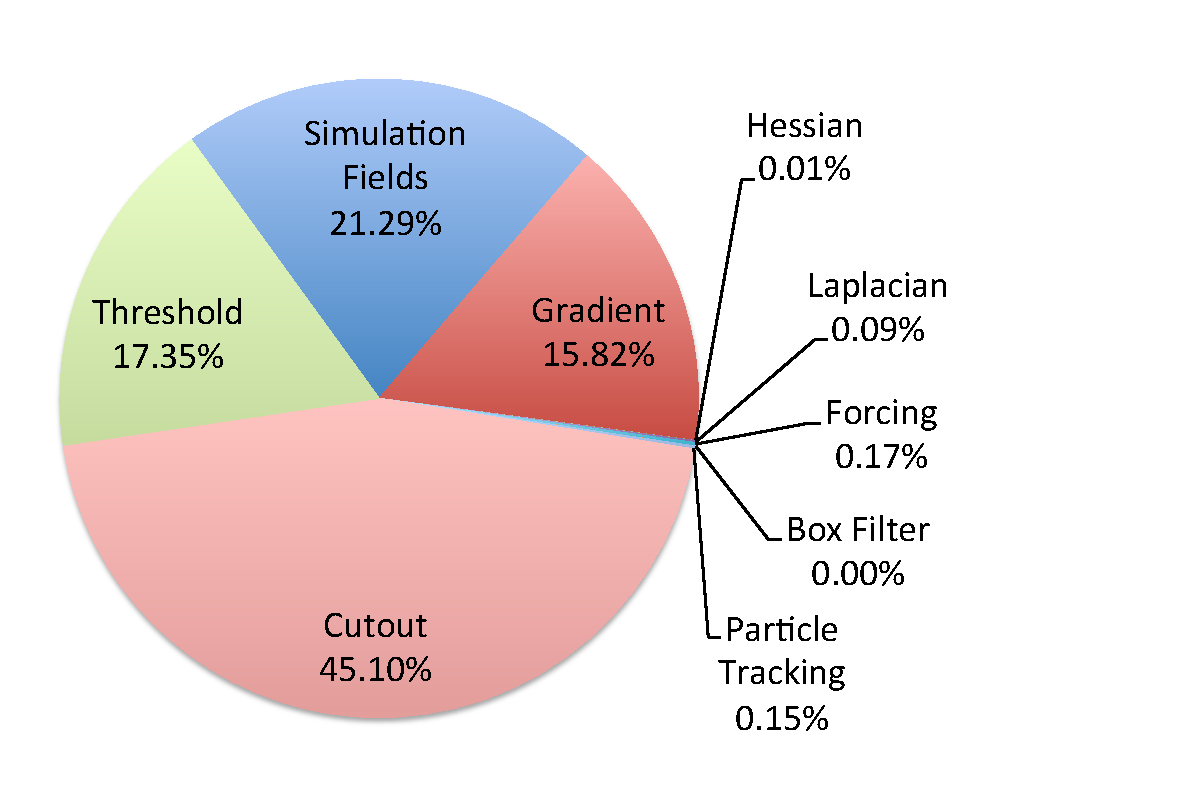
\includegraphics[width=0.49\textwidth]{jhtdb_total_per_query_type.pdf}\label{fig:points_per_type}}
\caption{Distribution of JHTDB queries and number of data points queried per query type.}
\label{fig:query_types}
\end{figure*}

JHTDB usage has grown steadily over the years with the addition of new datasets and expanded capabilities and performance. Figure \ref{fig:points_queried}
shows the total number of points queried per year since the JHTDB's inception in 2007 and the total number of queries submitted is shown in Figure
\ref{fig:queries}. As we can see there has been an exponential growth in the total number of data points queried over the past several years, mainly due to
new access methods, increased number of analysis functionalities and the addition of new datasets. 
The MHD dataset was released in 2011, the channel flow dataset
became public in 2013 and the mixing dataset was released in 2014. In 2011 the particle tracking functionality was implemented and made available, while
in 2012 the data cutout service went online. This new functionality has greatly increased the utility of the service. The data-intensive iterative process used to
track particles is much more efficiently executed near the data. On the other hand, the cutout service has provided an easy and efficient way for researchers to
obtain the raw simulation data if they so choose. 

Most queries submitted and evaluated by the JHTDB request the simulation field parameters and their spatial derivatives as can be seen in Figure
\ref{fig:queries_per_type}. The number of requests made through the cutout service is significantly smaller. However, in terms of the actual size of the requests
and the total amount of data retrieved, the cutout requests are a much larger slice of the pie as seen in Figure \ref{fig:points_per_type}. The recently introduced
threshold queries are another example of an extremely data-intensive task, which is efficiently performed by the database cluster. A single request for the 
number of points above a particular threshold usually examines up to the entire $1024^3$ or larger data volume of a simulation time-step. 
There have been only $\sim2000$ such queries executed so far, and yet over 1 trillion points have been examined by this query type alone.

\section{Immersive turbulence}
Using the JHTDB and accompanying access libraries and tools, scientists can immerse virtual sensors in the simulation, visualize turbulent phenomena, 
perform feature extraction and data mining. The data and the associated functionality are available on-demand and over the internet. This allows scientists 
to interact with the entire simulation data. Stationary sensors immersed in the flow report the simulation parameters or values of derived fields at particular 
locations, while particles can be allowed to flow both forward and backward in time along pathlines or along streamlines within a single time-step. 
We term this approach to computational science ``remote immersive analysis".

\begin{figure*}
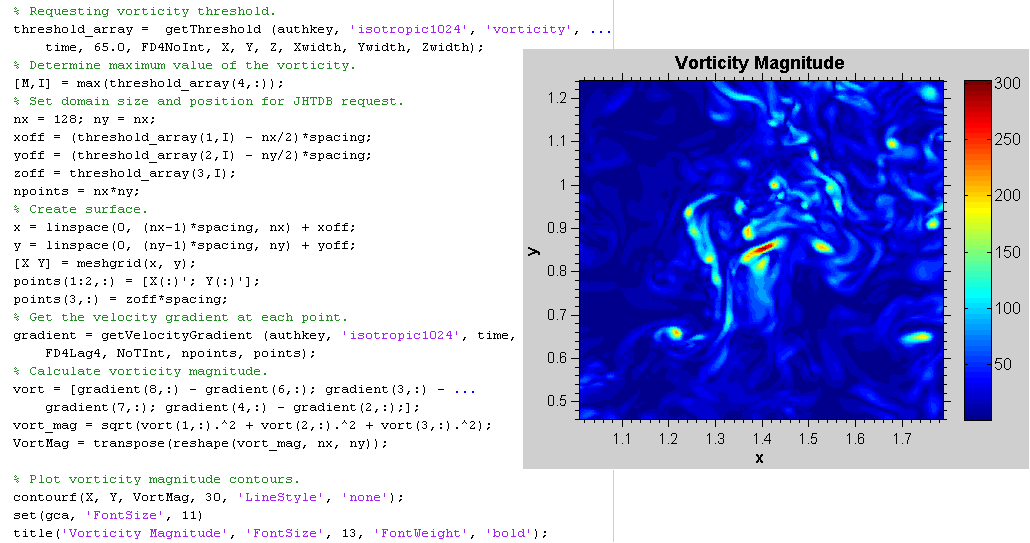
\includegraphics[width=1.0\textwidth]{vorticity.png}
\caption{Matlab script to examine the vorticity magnitude around a point with large vorticity in the isotropic turbulence dataset stored in the JHTDB.}
\label{fig:vorticity}
\end{figure*}

Figure \ref{fig:vorticity} shows an example of the remote immersive analysis approach to computational turbulence. The user extracts all locations within the
region of interest where the magnitude of the vorticity is above a prescribed threshold (65.0 in the example) from the isotropic turbulence dataset (making 
a call to the getThreshold Web-service method). He or she then generates a 2D planar patch with the location of maximum vorticity in the center and places
``virtual sensors" at each location using the dataset's gird spacing. He or she then requests the velocity gradient (making a call to the getVelocityGradient
Web-service method) at each of these locations and computes and plots the vorticity magnitude to yield the visualization shown. The results of the 
getThreshold and getVelocityGradient methods can be further analyzed depending on the particular needs of the user.

Many numerical simulations are canonical and have useful lifetimes of years or decades. Turbulence researchers have come to rely on the JHTDB to 
provide such canonical datasets and new ideas are tested on the service routinely. The scientific results that have emerged span the full breadth of 
turbulence research, from physical theory (e.g. turbulent dynamics of velocity gradients \cite{luethi2009expanding}), to engineering modeling 
(e.g. large-eddy simulation of wall-bounded flows \cite{gungor2010new}), to development of experimental techniques 
(e.g. particle-based measurements of very fine-scale flow structure \cite{lawson2014scanning}).
These are just a handful of the many examples showing the utility of the 
JHTDB and how it has enabled data-driven discovery.

\section{Conclusion}
We have described an open simulation laboratory for the study of turbulent phenomena, the JHTDB. It provides public access to high-quality turbulence 
numerical simulation data along with built-in analysis functionality. Scientists and the public as a whole can immerse sensors in the simulated flows, study
their evolution or the flow parameters. This can and has been done from around the world by researches that don't have access to supercomputing facilities
and/or large amounts of local storage and computational resources. The JHTDB is the manifestation of the ``remote immersive analysis" approach to 
computational science.

In the future we plan on expanding the capabilities of the JHTDB through adding interactive visualization capabilities, custom server side computations and
the ability	to generate and store derived datasets. Visualization software will run in server
mode on our servers and will allow remote client connections. We are also exploring Web interfaces for such visualization software, which will allow users
to perform visualizations through a Web-browser. By integrating the JHTDB with existing technology developed for the Sloan Digital Sky Survey (SDSS), such
as CasJob and MyDB \cite{LiThakar} we will be able to provide server-side storage for our users. The results of data-intensive computations and iterative 
workflows can be stored in this server-side storage to be downloaded or interacted with later. This will also allow for the generation of derived datasets (e.g.
filtered versions of the original datasets), which can then be used through the existing Web-services. This will also allow for interacting with the data in new
and different ways.

\vfill
\newpage
 
\bibliography{jhtdb}
\vfill

\newpage
   
 \end{document}



 


